\documentclass[a4paper,12pt]{article} %размер бумаги устанавливаем А4, шрифт 12пунктов
\usepackage[utf8]{inputenc}
\usepackage{csquotes}
\usepackage[english,russian]{babel}%используем русский и английский языки с переносами
\usepackage{biblatex}
\bibliography{refs}
\usepackage{amssymb,amsfonts,mathtext,enumerate,float} %подключаем нужные пакеты расширений
\usepackage{textcomp}
\usepackage{adjustbox}
\usepackage{graphicx} %хотим вставлять в диплом рисунки?
\makeatletter
\makeatother
\usepackage{sagetex}
\usepackage{geometry} % Меняем поля страницы
\geometry{left=2cm}% левое поле
\geometry{right=1.5cm}% правое поле
\geometry{top=1cm}% верхнее поле
\geometry{bottom=2cm}% нижнее поле
\usepackage{tabularx}
\usepackage{threeparttable}
\usepackage{epstopdf}
\usepackage{amsmath} %отображение математической нотации
\usepackage{caption, subcaption} %подписи}
\usepackage{indentfirst}%отступ вначале параграфа
\usepackage{pscyr}

\captionsetup[table]{labelsep = endash, singlelinecheck=false}
\captionsetup[figure]{name = Рисунок, labelformat=simple, labelsep = endash}


\begin{document}


\newcommand\tline[2]{$\underset{\text{#1}}{\text{\underline{\hspace{#2}}}}$}
\newcommand\nameLine[3]{$\underset{\text{#1}}{\text{\underline{\text{#2}\hspace{#3}}}}$}

\begin{titlepage}
	\centering
	{\fontsize{12pt}{5cm}\selectfont \bfseries Министерство образования и науки Российской Федерации} \\ \vspace{0.5cm}
	{\fontsize{7pt}{5cm}\selectfont ФЕДЕРАЛЬНОЕ ГОСУДАРСТВЕННОЕ АВТОНОМНОЕ ОБРАЗОВАТЕЛЬНОЕ УЧРЕЖДЕНИЕ ВЫСШЕГО ПРОФЕССИОНАЛЬНОГО ОБРАЗОВАНИЯ} \\ 
	\vspace{1cm}
	{\fontsize{12pt}{5cm}\selectfont \bfseries САНКТ-ПЕТЕРБУРГСКИЙ УНИВЕРСИТЕТ ИНФОРМАЦИОННЫХ ТЕХНОЛОГИЙ, МЕХАНИКИ И ОПТИКИ} \\ \vspace{1.5cm}
	
	{\fontsize{14pt}{5cm}\selectfont Кафедра \hspace{1cm} \underline{Систем Управления и Информатики}  \hspace{1cm} Группа \underline{Р3340}} \\
	
	\vspace{2cm}
	
	{\fontsize{20pt}{5cm}\selectfont \bfseries Лабораторная работа №9} \\
	{\fontsize{20pt}{5cm}\selectfont \bfseries “Экспериментальное построение частотных характеристик типовых динамических звеньев”} \\
	\vspace{0.2cm}
	{\fontsize{14pt}{5cm}\selectfont Вариант - 10} \\
	
	\vspace{1.5cm}
	
	\flushleft
	{Выполнилa \hspace{1.8cm} \nameLine{(фамилия, и.о.)}{Ким А. А.}{7cm} (подпись)} \\
	
	\vspace{2cm}
	
	{Проверил \hspace{2cm} \tline{(фамилия, и.о.)}{9cm} (подпись)} \\
	
	\vspace{5cm}
	
	"\underline{\hspace{0.7cm}}"\hspace{0.2cm}\underline{\hspace{2cm}}\hspace{0.2cm}20\underline{\hspace{0.7cm}}г. \hspace{2cm} Санкт-Петербург, \hspace{2cm} 20\underline{\hspace{0.7cm}}г. \\ \vspace{1cm}
	
	Работа выполнена с оценкой \hspace{1cm} \underline{\hspace{8cm}} \\ 
	\vspace{1cm}
	Дата защиты "\underline{\hspace{0.7cm}}"\hspace{0.2cm}\underline{\hspace{2cm}}\hspace{0.2cm}20\underline{\hspace{0.7cm}}г.
\end{titlepage}
\setcounter{page}{2}

\paragraph{Цель работы:}Изучение математических моделей и исследование характеристик исполнительного устройства, построенного на основе пьезоэлектрического двигателя микроперемещений.
\paragraph{Исходные данные.}

Исходные данные для выполнения работы приведены в таблице \ref{Tab1}.
\begin{table}[h!]
	\renewcommand{\arraystretch}{1.3} %строки
	\renewcommand{\tabcolsep}{0.3cm} %столбцы
	\centering
	\begin{threeparttable}
    \caption{Исходные данные}
    \begin{tabular}{|c|c|c|c|c|c|c|c|}
    \hline $C_P$ & m & $K_O$ & $K_d$ & $T_u$ & $F_B$ & $U_{Pm}$ & $U_m$\\
    Н/м & кг & H/B & Нc/м & мc & H & B & B\\
    \hline $4,2\cdot10^6$ & 0,25 & 10 & $0,75\cdot10^2$ & 0,15 & 3 & 300 & 10\\
    \hline
    \end{tabular} 
    \label{Tab1}
    \end{threeparttable}
\end{table}

$K_u=U_{Pm}/U_m=300/10=30$
\par
Коэффициенты передачи $K_u^{-1}, K_F, K_V, K_X$ определяются так, чтобы обеспечить соответствие максимального значения измеряемого сигнала уровню 10 В на выходе измерительного устройства.\\ 
$K_u^{-1} = 0,0333$\\
$K_F = 0,005$\\
$K_V = 4,2$\\
$K_X = 14000$

\newpage
\section{Математическое моделирование модели пьезоэлектрического исполнительного устройства}	 
На основе структурной схемы, представленной на рисунке \ref{structScheme}, составим схему моделирования ПД (рисунок \ref{cxema1}).
\begin{figure}[ht!]
	\centering
	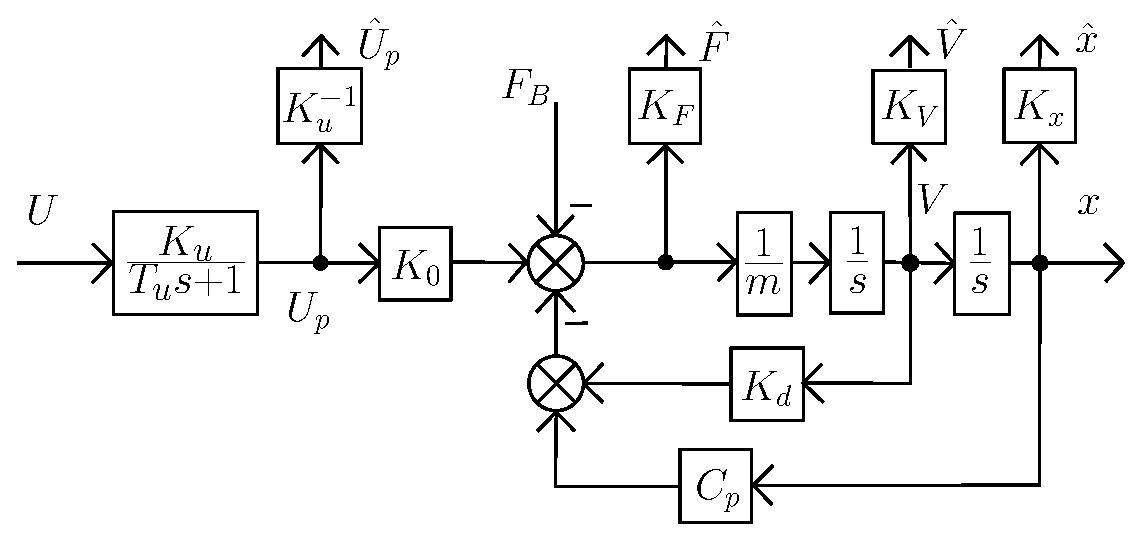
\includegraphics[width = 0.8 \textwidth]{scheme/structScheme}
	\caption{Структурная схема пьезоэлектрического исполнительного устройства}
	\label{structScheme}
\end{figure}
\begin{figure}[ht!]
	\centering
	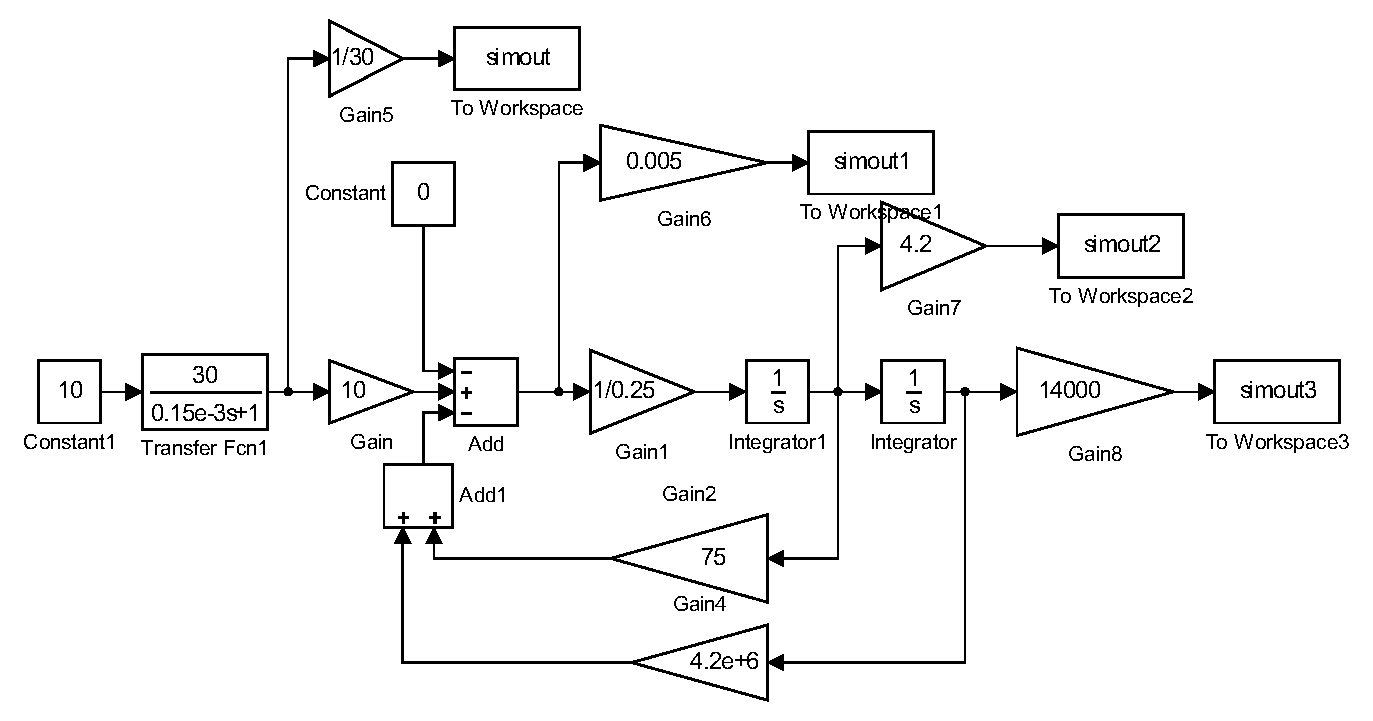
\includegraphics[width = \textwidth]{scheme/scheme1}
	\caption{Схема моделирования ПД}
	\label{cxema1}
\end{figure}

Построим графики переходных процессов при $F_B=0$H и U=10B (рисунок \ref{UFVX0}):
\begin{figure}[H]
	\centering
	\begin{subfigure}[b]{0.48\textwidth}
	    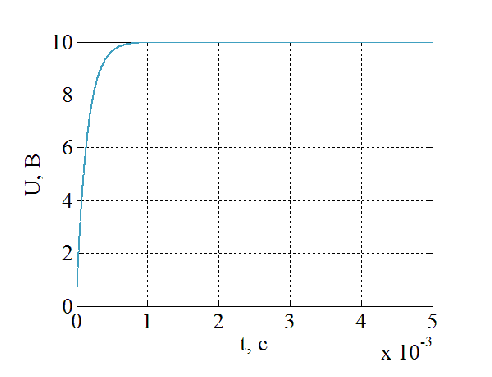
\includegraphics[width = \textwidth]{scheme/U0}
	\end{subfigure}
	\hfill
	\begin{subfigure}[b]{0.48\textwidth}
		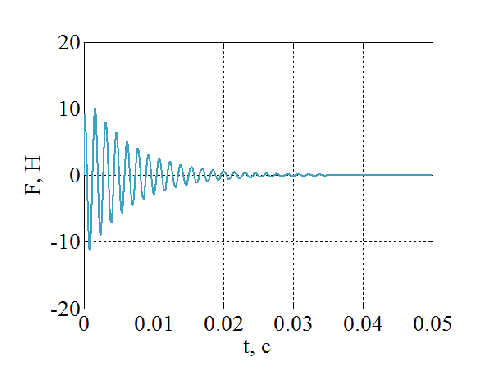
\includegraphics[width = \textwidth]{scheme/F0}
	\end{subfigure}
	\begin{subfigure}[b]{0.48\textwidth}
		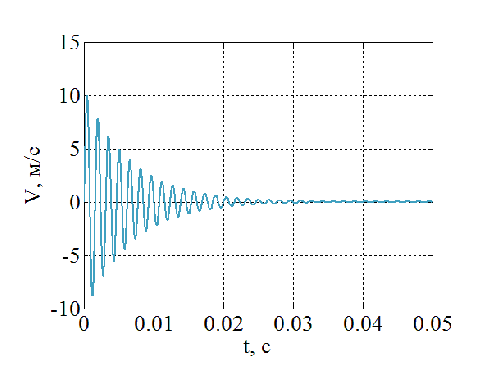
\includegraphics[width = \textwidth]{scheme/V0}
	\end{subfigure}
	\hfill
	\begin{subfigure}[b]{0.48\textwidth}
		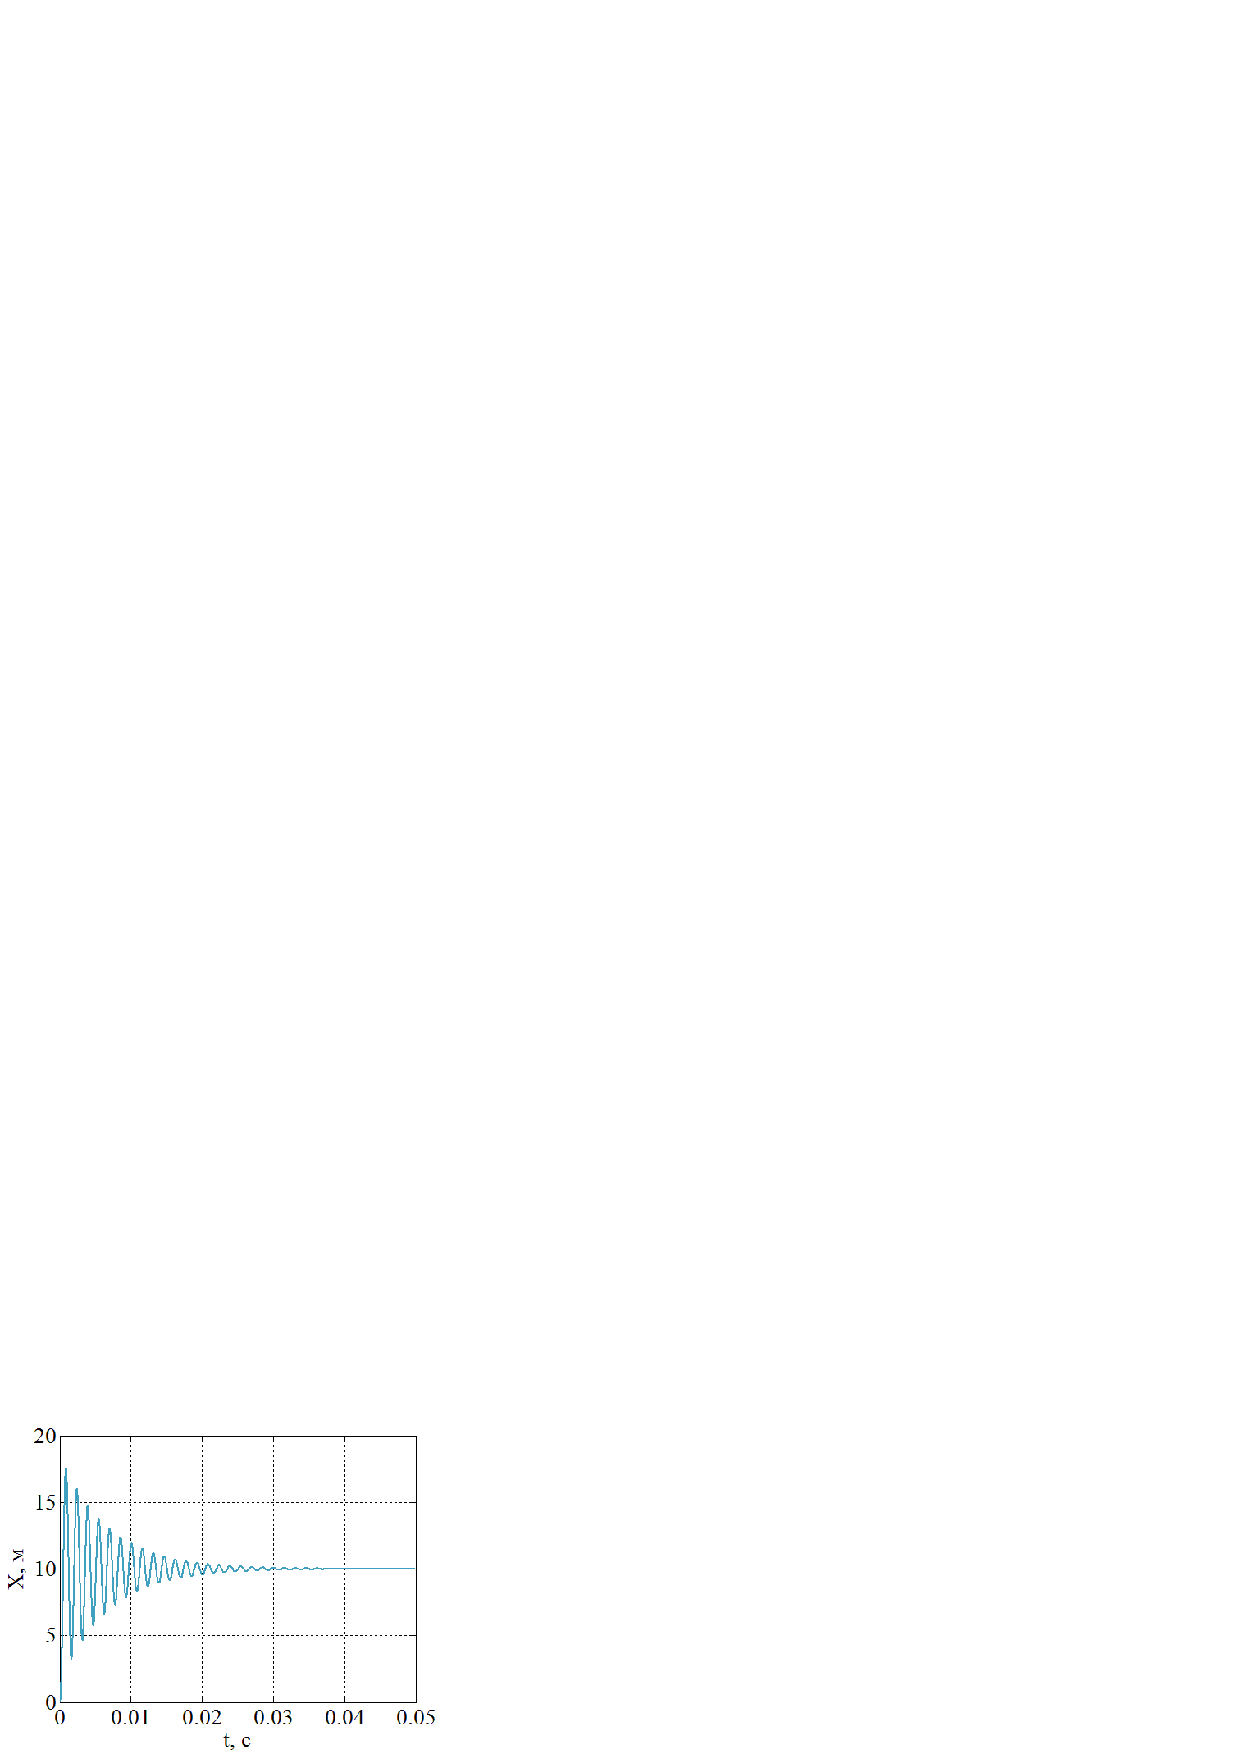
\includegraphics[width = \textwidth]{scheme/X0}
	\end{subfigure}
	\caption{Графики переходных процессов при $F_B=0$H и U=10B}
	\label{UFVX0}
\end{figure}

\newpage
\section{Исследование влияния массы нагрузки m на вид переходных процессов}
Диапазон изменения массы нагрузки m: $\pm 50\%$  от заданного значения. Графики переходных процессов представлены на рисунке \ref{UFVX1}.
\begin{figure}[H]
	\centering
	\begin{subfigure}[b]{0.48\textwidth}
	    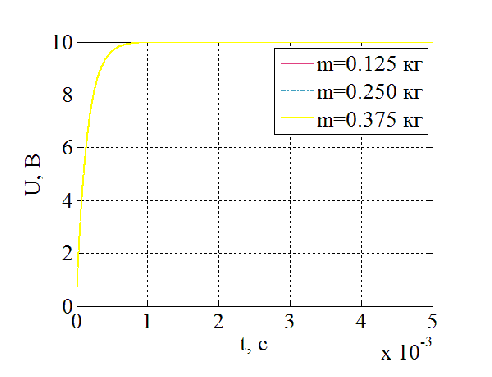
\includegraphics[width = \textwidth]{scheme/U1}
	\end{subfigure}
	\hfill
	\begin{subfigure}[b]{0.48\textwidth}
		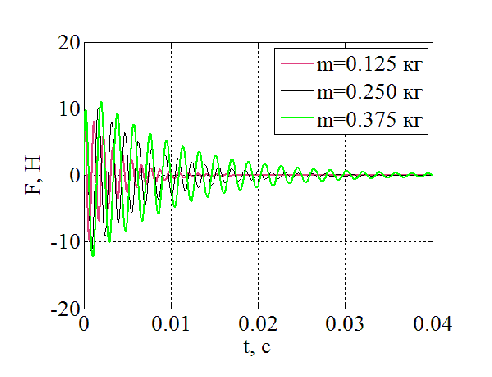
\includegraphics[width = \textwidth]{scheme/F1}
	\end{subfigure}
	\begin{subfigure}[b]{0.48\textwidth}
		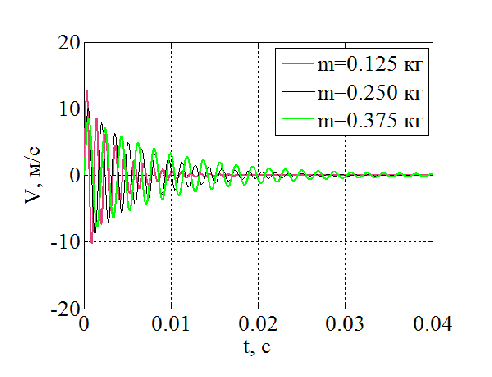
\includegraphics[width = \textwidth]{scheme/V1}
	\end{subfigure}
	\hfill
	\begin{subfigure}[b]{0.48\textwidth}
		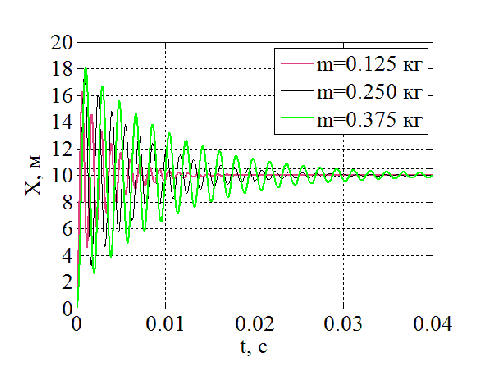
\includegraphics[width = \textwidth]{scheme/X1}
	\end{subfigure}
	\caption{Графики переходных процессов при различных значениях m}
	\label{UFVX1}
\end{figure}

По временным диаграммам определим время переходного процесса $t_\text{П}$, величину перерегулирования $\sigma$ и установившееся значение $X_y$. Занесём результаты в таблицу \ref{Tab2}.
\begin{table}[h!]
	\renewcommand{\arraystretch}{1.3} %строки
	\renewcommand{\tabcolsep}{0.3cm} %столбцы
	\centering
	\begin{threeparttable}
    \caption{Характеристики системы при меняющейся массе нагрузки}
    \begin{tabular}{|c|c|c|c|}
    \hline m, \text{кг} & $t_\text{П}, \text{мс}$ & $\sigma, \%$ & $X_y$\\
    \hline 0,125 & 0.010 & 61,8 & 10 \\
    \hline 0,250 & 0.019 & 75 & 10 \\
    \hline 0,375 & 0.030 & 62 & 10 \\
    \hline
    \end{tabular} 
    \label{Tab2}
    \end{threeparttable}
\end{table}

\newpage
\section{Исследование влияния $T_u$ на вид переходных процессов}
Изменение $T_u$ в сторону увеличивая исходного значения постоянной времени в 2, 4 и 6 раз. Графики переходных процессов представлены на рисунке \ref{UFVX2}.
\begin{figure}[H]
	\centering
	\begin{subfigure}[b]{0.48\textwidth}
	    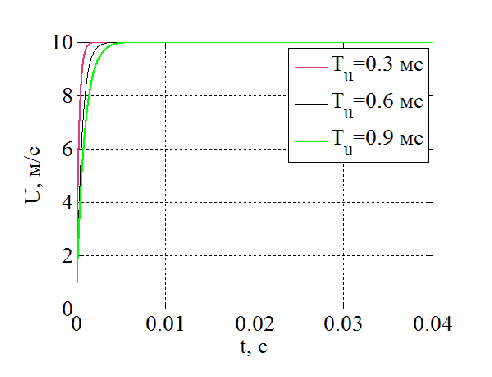
\includegraphics[width = \textwidth]{scheme/U2}
	\end{subfigure}
	\hfill
	\begin{subfigure}[b]{0.48\textwidth}
		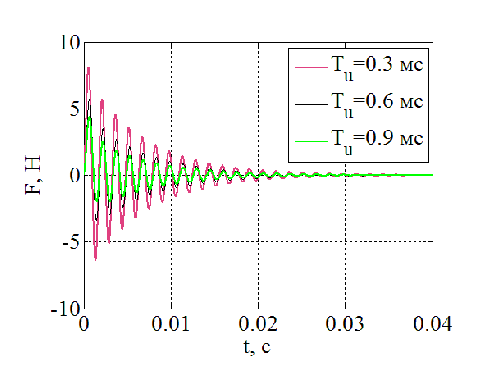
\includegraphics[width = \textwidth]{scheme/F2}
	\end{subfigure}
	\begin{subfigure}[b]{0.48\textwidth}
		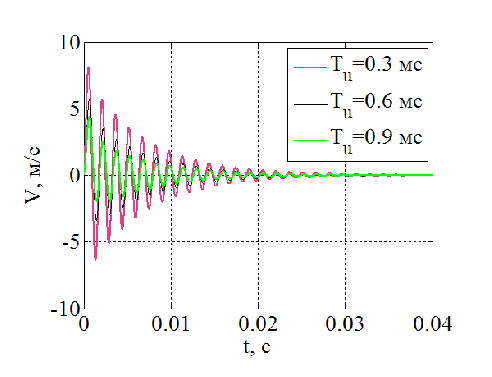
\includegraphics[width = \textwidth]{scheme/V2}
	\end{subfigure}
	\hfill
	\begin{subfigure}[b]{0.48\textwidth}
		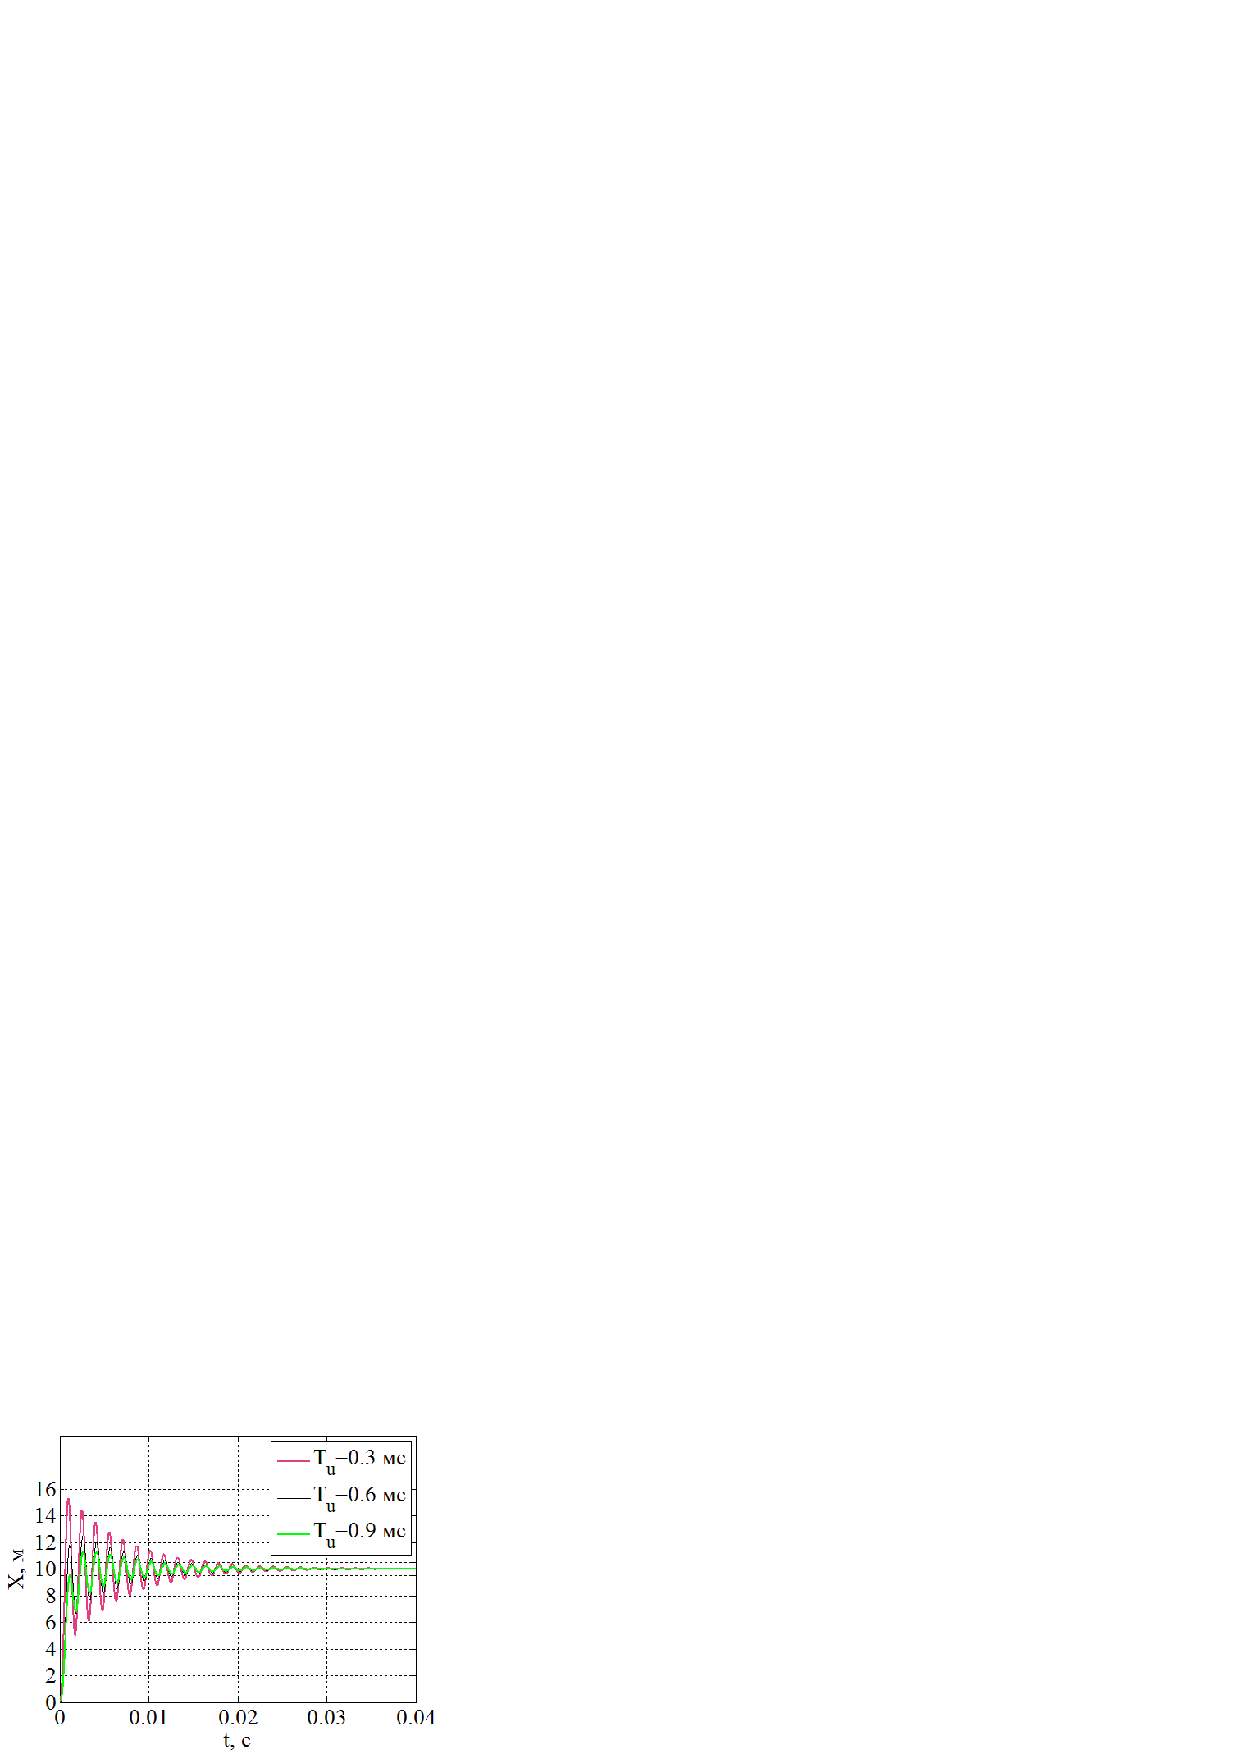
\includegraphics[width = \textwidth]{scheme/X2}
	\end{subfigure}
	\caption{Графики переходных процессов при различных значениях $T_u$}
	\label{UFVX2}
\end{figure}
По результатам моделирования определим время переходных процессов $t_\text{П}$, величину перерегулирования $\sigma$ и установившееся значение $X_y$. Занесём результаты в таблицу \ref{Tab3}.
\begin{table}[h!]
	\renewcommand{\arraystretch}{1.3} %строки
	\renewcommand{\tabcolsep}{0.3cm} %столбцы
	\centering
	\begin{threeparttable}
    \caption{Характеристики системы при меняющейся постоянной времени}
    \begin{tabular}{|c|c|c|c|c|c|c|}
    \hline $T_u$, \text{с} & $t_\text{П}, \text{мс}$ & $\sigma, \%$ & $X_y$ & $s_1$ & $s_2$ & $s_3$\\
    \hline 0,3 & 0,016 & 55  &  10 & -3333,33 & -150-i4096,03 & -150+i4096,03\\
    \hline 0,6 & 0,013 & 25   &  10 & -1666,67 & -150-i4096,03 & -150+i4096,03\\ 
    \hline 0,9 & 0,012 & 10   &  10 & -1111,11 & -1500-i4096,03 & -150+i4096,03\\ 
    \hline
    \end{tabular} 
    \label{Tab3}
    \end{threeparttable}
\end{table}

Чтобы рассчитать значения корней характеристического уравнения получим передаточную функцию. Для этого будем рассматривать исполнительное пьезоэлектрическое устройство как упругую механическую систему. В этом случае математическая модель может быть получена на основе уравнения баланса сил в пьезодвигателе:  
\begin{equation} 
    F_y = F_O + F_\text{Д} + F_d + F_B,
    \label{F}
\end{equation}
где $F_y=C_px$ --- усилие упругой деформации ПД, $F_O=K_OU_p$ --- усилие, вызванное обратным пьезоэффектом, $F_\text{Д}=-m\displaystyle{\frac{d^2x}{dt^2}}$ --- динамическое усилие в ПД, $F_d=-K_d\displaystyle{\frac{dx}{dt}}$ --- демпфирующее усилие, обусловленное механическими потерями, $F_B$ --- внешнее воздействие, x --- перемещение, $C_p$ --- коэффициент упругости, $K_O$ --- коэффициент обратного пьезоэффекта, $U_p$ --- напряжение на электродах ПД, m --- масса перемещаемой нагрузки, $K_d$ --- коэффициент демпфирования.\par
Подставив перечисленные равенства в уравнение (\ref{F}), получим:
\begin{equation} 
    m\ddot{x} + K_d\dot{x} + C_px = K_OU_p + F_B
    \label{F1}
\end{equation}
\par Составленная по уравнению (\ref{F1}) передаточная функция будет выглядеть следующем образом:
\begin{equation} 
    W_{\text{ВУ}}(s)=\frac{K_OU_p + F_B}{ms^2 + K_ds + C_p}
    \label{FVU}
\end{equation}
\par Управление ПД осуществляется от высоковольтного усилителя, который, в нашем случае, описывается апериодическим звеном первого порядка:
\begin{equation} 
    W(s)=\frac{K_u}{T_us + 1}
\end{equation}
\par Исходя из того, что ВУ и ПД соединены последовательно, имеем передаточную следующую функцию:
\begin{equation} 
    W(s)=\frac{K_u(K_OU_p + F_B)}{(T_us + 1)(ms^2 + K_ds + C_p)}
\end{equation}
\par Найдем корни характеристического уравнения для всех сочетаний параметров и запишем результат в таблицу \ref{Tab3}.

\newpage
\section{Исследование влияния коэффициента упругости $C_p$ на вид переходных процессов}
Исследования проводились при значениях коэффициента упругости 0,5$C_p$ и 2$C_p$ при $F_B=3$H и U=0B. Графики переходных процессов изображены на рисунке \ref{VX3}.
\begin{figure}[H]
	\centering
	\begin{subfigure}[b]{0.48\textwidth}
	    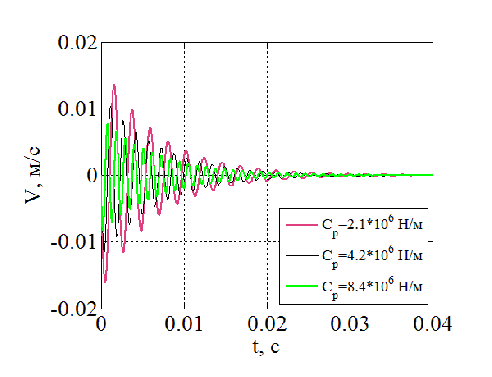
\includegraphics[width = \textwidth]{scheme/V3}
	\end{subfigure}
	\hfill
	\begin{subfigure}[b]{0.48\textwidth}
		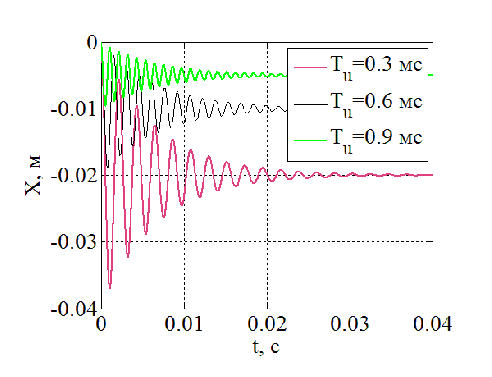
\includegraphics[width = \textwidth]{scheme/X3}
	\end{subfigure}
	\caption{Графики переходных процессов при различных значениях коэффициента упругости}
	\label{VX3}
\end{figure}



\newpage
\section{Построение асимптотической ЛАЧХ исполнительного устройства}
Представим передаточную функцию (\ref{FVU}) в виде колебательного звена:
\begin{equation} 
    W(s) = \frac{\displaystyle{\frac{K_0}{C_p}}}{\displaystyle{\frac{m}{C_p}}s^2 + \frac{K_d}{C_p}s + 1}.
\end{equation}

Асимптотическая логарифмическая амплитудная характеристика будет иметь нулевой наклон на уровне 
\begin{equation} 
   20\lg\displaystyle{\frac{K_0}{C_p}} = 20\lg \displaystyle{\frac{10}{4,2\cdot10^6}} = -112,4 \text{дБ}
\end{equation}
до сопрягающей частоты 
\begin{equation} 
	\omega_c = \sqrt{\displaystyle{\frac{C_p}{m}}} = \sqrt{\displaystyle{\frac{0,5\cdot10^8}{0,3}}} = 4099 \text{рад/с}.
\end{equation}
\par
После сопрягающей частоты график пойдёт под наклоном в -40 дБ/дек. Таким образом асимптотическая ЛАЧХ будет выглядить так как показано на рисунке \ref{L}:
\begin{figure}[H]
	\centering
	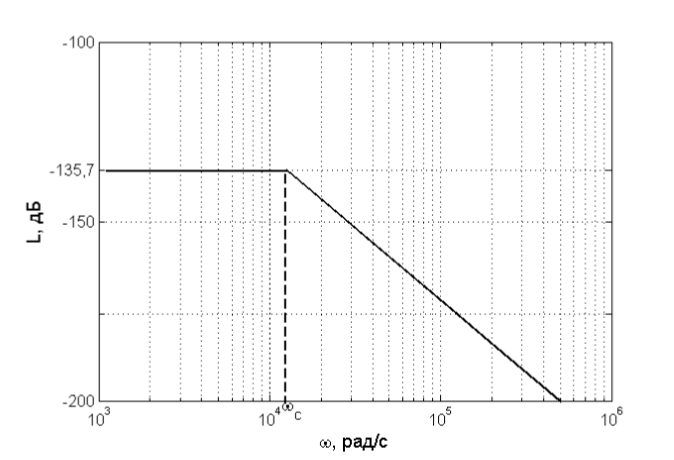
\includegraphics[width = \textwidth]{scheme/L}
	\caption{Асимптотическая ЛАЧХ исполнительного устройства}
	\label{L}
\end{figure}

\newpage
\begin{center}
	\section*{Вывод}
\end{center}
\par
В ходе лабораторной работы было проведено исследование пьезоэлектрического устройства. 
Были выявлены изменения в переходных процессах системы путём изменения таких параметров как масса нагрузки, постоянная времени, коэффициент упругости.\par
Как видно из таблицы \ref{Tab2} при уменьшении массы нагрузки установившееся значение перемещения остаётся постоянным, а значение времени переходного процесса и перерегулирования уменьшается. \par
При исследовании влияния постоянной времени вольтного усилителя было показано, что её увеличение ведёт к уменьшению перерегулирования, а также к уменьшению одного из корней характеристического уравнения, что можно увидеть в таблице \ref{Tab3}.\par
Из графиков (рисунок \ref{VX3}) видно, что при увеличении значения коэффициента упругости пьезоэлемента увеличивается установившееся значение перемещения пьезокерамических пластин.

\end{document}
